\documentclass[a4paper]{article}
\usepackage[utf8]{vntex}
\usepackage[english]{babel}
\usepackage[utf8]{inputenc}
\usepackage{amsmath,graphicx,xcolor,booktabs,array,indentfirst}
\usepackage[margin=25mm,headheight=32pt,headsep=8mm]{geometry}
\usepackage{fancyhdr,listings}
\usepackage[colorlinks=true,linkcolor=black,citecolor=black,urlcolor=blue]{hyperref}
\setlength{\parindent}{1cm}
\setlength{\parskip}{0pt}
\setlength{\emergencystretch}{2em}
\raggedbottom
\clubpenalty=10000
\widowpenalty=10000
\pagestyle{fancy}
\fancyhf{}
\fancyhead[R]{%
\begin{tabular}{@{}r@{\hspace{2mm}}c@{}}
\begin{tabular}{@{}r@{}}
\small Ho Chi Minh City University of Technology\\
\small Faculty of Computer Science and Engineering
\end{tabular}&\raisebox{-2mm}{
\includegraphics[width=8mm]{hcmut_logo.png}}
\end{tabular}}
\fancyfoot[L]{\footnotesize Microprocessors--Microcontrollers Laboratory (CO3010)}
\fancyfoot[R]{\footnotesize\thepage}
\renewcommand{\headrulewidth}{0.3pt}
\definecolor{codeblue}{RGB}{0,83,160}
\definecolor{codebg}{RGB}{247,248,250}
\lstset{language=C,basicstyle=\ttfamily\small,
keywordstyle=\color{codeblue}\bfseries,stringstyle=\color{red!60!black},
numbers=left,numberstyle=\tiny\color{gray},numbersep=7pt,
frame=single,rulecolor=\color{gray!40},backgroundcolor=\color{codebg},
breaklines=true,breakatwhitespace=false,keepspaces=true,
columns=fullflexible,tabsize=4,showstringspaces=false,
captionpos=t,aboveskip=10pt,belowskip=10pt,xleftmargin=12pt,
framexleftmargin=3pt}
\newcommand{\code}[1]{\texttt{\detokenize{#1}}}
\newcommand{\topic}[1]{\subsection{#1}}
\begin{document}
\hypersetup{pageanchor=false}
\begin{titlepage}
\centering
{\large VIETNAM NATIONAL UNIVERSITY HO CHI MINH CITY\par}
\vspace{3mm}
{\large HO CHI MINH CITY UNIVERSITY OF TECHNOLOGY\par}
\vspace{3mm}
{\large FACULTY OF COMPUTER SCIENCE AND ENGINEERING\par}
\vspace{15mm}

\includegraphics[width=4cm]{hcmut_logo.png}\par
\vspace{13mm}
\par{\Large\bfseries Microprocessors--Microcontrollers Laboratory\par}
{\Large\bfseries (CO3010)\par}
\vspace{8mm}
\rule{\textwidth}{0.5pt}\par
\vspace{6mm}
{\Large\bfseries Laboratory Report\par}
\vspace{6mm}
{\LARGE\bfseries LAB 03\par}
\vspace{4mm}
{\Large\bfseries Buttons, Switches, and Traffic-Light Control\par}
\vspace{6mm}
\rule{\textwidth}{0.5pt}\par
\vspace{18mm}
\begin{tabular}{rl}
Advisor: & Phan Văn Sỹ\\[3mm]
Student: & Nguyễn Cáp Quốc Khánh\\[3mm]
Student ID: & 2452500\\[3mm]
Class: & CC03
\end{tabular}
\vfill
{\small HO CHI MINH CITY, NOVEMBER 2026\par}
\end{titlepage}
\hypersetup{pageanchor=true}
\pagenumbering{roman}
\begingroup
\small
\setcounter{tocdepth}{2}
\tableofcontents
\endgroup
\clearpage
\listoffigures
\listoftables
\clearpage
\pagenumbering{arabic}

\section*{Overview}
\addcontentsline{toc}{section}{Overview}
This laboratory develops a configurable traffic-light controller using three
active-low buttons, twelve traffic LEDs, and four seven-segment displays.
The input driver filters mechanical contact bounce and records button events.
A finite state machine interprets those events, controls the traffic phases,
and updates display values. Periodic interrupt services refresh the displays
and sample the buttons independently of the foreground application.

The four operating modes are normal operation, red-duration adjustment,
amber-duration adjustment, and green-duration adjustment. MODE selects a mode,
INC changes a candidate duration, and SET commits it. Separating the candidate
value from the active settings permits a user to inspect an adjustment before
it changes normal operation. The STM32 GPIO and timer interfaces are accessed
through HAL functions\cite{stm32,hal}; Keil and Proteus provide development and
circuit-simulation facilities\cite{keil,proteus}.

The symbol Y and the source variable \code{yellow_time} refer to the amber
interval. NS denotes the North--South road pair and EW the East--West pair.
Opposite directions share their color commands, so six control signals drive
twelve physical traffic LEDs. Excerpts below show the application logic;
generated initialization is included only when it explains a required setting.

\topic{Input, processing, and output model}

The application follows a three-stage information path. GPIO inputs first
become filtered electrical states, then become discrete button events. The
foreground state machine interprets those events using the current mode and
committed durations. Output functions finally translate numerical values and
color selections into GPIO levels. A low electrical level, a press event, and
a request to change mode are therefore three different concepts. Keeping them
separate prevents a held switch from being interpreted as a new MODE command
on every pass through the main loop.

Two time scales operate simultaneously. User-interface sampling and display
refresh require intervals of milliseconds, while traffic phases last seconds.
Neither a phase countdown nor a user's editing activity should interrupt the
display refresh. The implementation consequently retains periodic interrupt
services while the foreground performs short state-machine operations.
The four editing specifications use the same two road display pairs and the
same three buttons, which makes state-dependent interpretation essential.


\clearpage
\section{Exercise 1: Finite state machine}

\topic{Design idea and mode transitions}
The controller contains two related state machines. The outer state machine
selects the operating mode. Within mode 1, a four-phase state machine produces
the traffic sequence. Editing modes suspend the normal sequence and blink
only the selected color on all approaches. A MODE press advances once through
\(1\rightarrow2\rightarrow3\rightarrow4\rightarrow1\).
The diagram shows the mode transitions; INC and SET are self-transitions
within an editing mode because they change data without changing mode.

\begin{figure}[htbp]
\centering
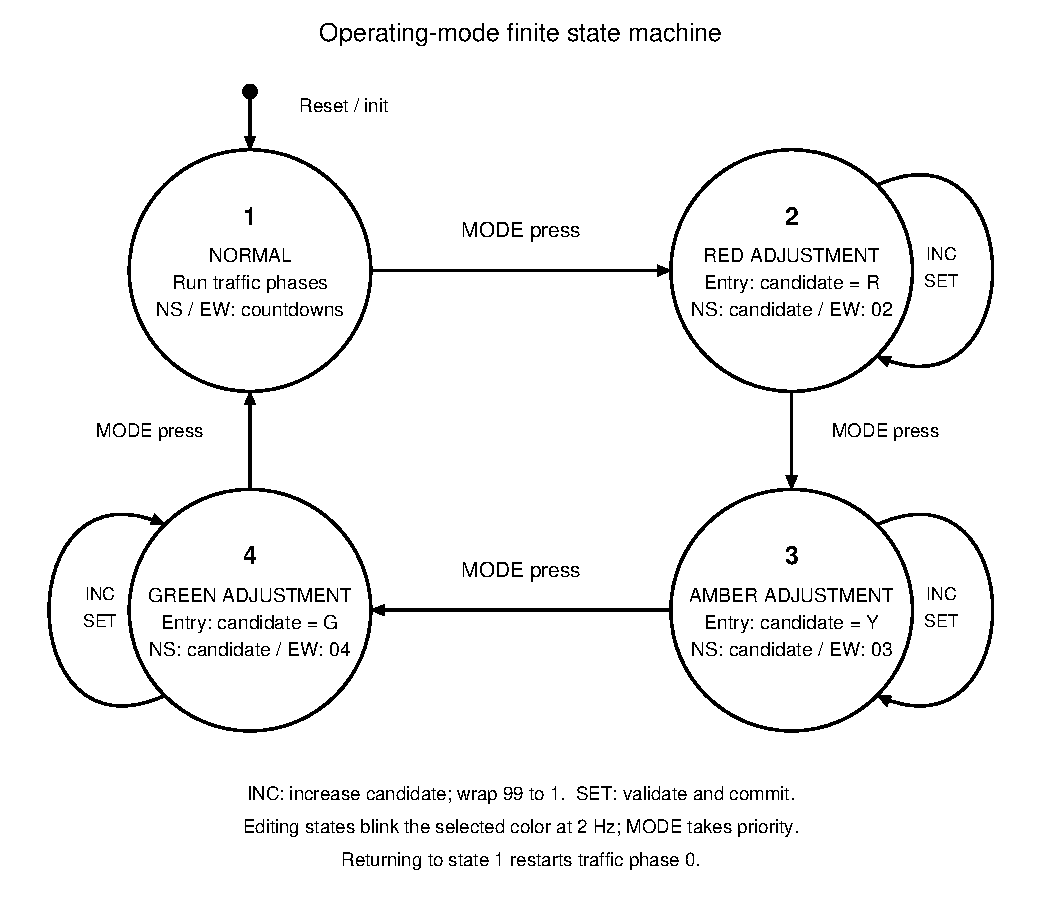
\includegraphics[width=0.96\textwidth]{fsm_modes.pdf}
\caption{Operating-mode FSM with entry actions and editing-mode events.}
\label{fig:modes}
\end{figure}

\topic{State variables, events, and entry actions}

A state machine is described by its current state, input event, transition
condition, and resulting action. Here \code{mode} is the outer state variable.
A filtered MODE press is its transition event. \code{change_mode()} increments
the state and wraps a value greater than four back to one. The normal state
enters through \code{start_normal()}, whereas each editing state loads the
duration associated with its color. Loading on entry prevents the displayed
candidate from accidentally carrying over from a different color.

The candidate \code{edit_value} is distinct from \code{red_time},
\code{yellow_time}, and \code{green_time}. INC updates the candidate;
SET updates committed configuration after validation. This is a small
transaction: selection, adjustment, confirmation. The selected mode remains
unchanged after INC or SET, so these are self-transitions in the mode FSM.
The circular arrows labeled INC and SET in Figure~\ref{fig:modes} show
these self-transitions. Blinking is also a repeated action within the current state,
not a transition to another editing mode.

The second state variable, \code{phase}, is meaningful during mode 1 only.
Keeping mode and phase separate avoids creating a large collection of mixed
states such as ``red-edit while EW-green.'' Entering an editing mode replaces
normal traffic outputs with a color demonstration; returning to normal starts
a new phase sequence using the latest committed durations.


\topic{Normal phases and timing relationship}
The initial durations are \(R=5\), \(Y=2\), and \(G=3\) seconds.
Each road remains red while the other road completes green and amber, giving
\(R=G+Y\). One complete intersection cycle lasts \(2(G+Y)=10\) seconds.
No normal-operation phase commands both crossing roads green; editing
modes intentionally blink all LEDs of the selected color. The phase index wraps after phase 3.
\begin{table}[htbp]\centering
\caption{Normal-state outputs and entry countdown values}
\begin{tabular}{ccccc}\toprule
Phase & NS color & EW color & NS display & EW display\\\midrule
0 & Green & Red & G & R\\
1 & Amber & Red & Y & Y\\
2 & Red & Green & R & G\\
3 & Red & Amber & Y & Y\\\bottomrule
\end{tabular}\end{table}
The second red countdown is loaded as Y at entry to phase 1 because the
opposite green interval has already elapsed: \(R-G=Y\). The same reasoning
applies to phase 3. Transition decisions use the currently green or amber
road's countdown, not two independent phase changes.

\par\noindent\begin{minipage}{\linewidth}
\begin{lstlisting}[caption={Traffic phase entry actions}]
static void show_phase(void)
{
    switch (phase)
    {
        case 0:
            ns_count = green_time;
            ew_count = red_time;
            TrafficLight_Init(NS_GREEN, EW_RED);
            break;
        case 1:
            ns_count = yellow_time;
            ew_count = yellow_time;
            TrafficLight_Init(NS_YELLOW, EW_RED);
            break;
        case 2:
            ns_count = red_time;
            ew_count = green_time;
            TrafficLight_Init(NS_RED, EW_GREEN);
            break;
        case 3:
            ns_count = yellow_time;
            ew_count = yellow_time;
            TrafficLight_Init(NS_RED, EW_YELLOW);
            break;
    }
    set_display(ns_count, ew_count);
}
\end{lstlisting}
\end{minipage}\par

\clearpage
\topic{Deriving the phase timing invariant}
\begin{figure}[!ht]
\centering
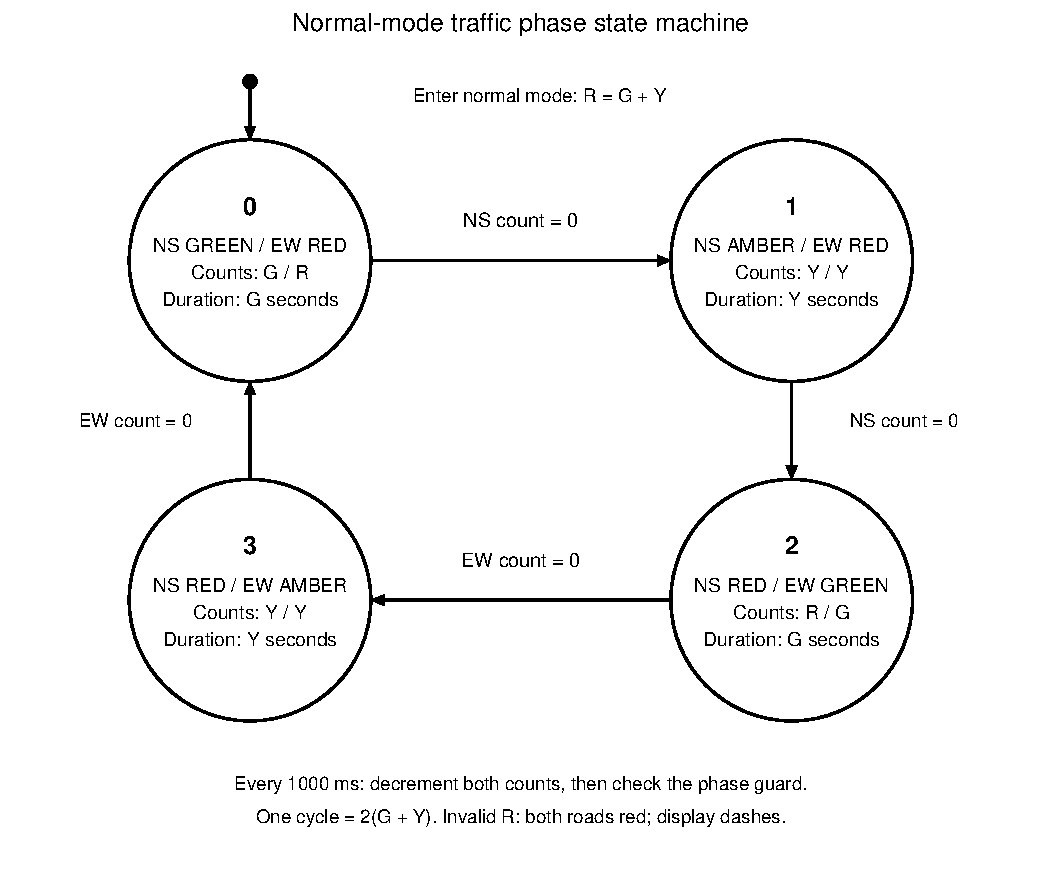
\includegraphics[width=0.85\textwidth]{fsm_phases.pdf}
\caption{Normal-operation FSM; guards are checked after the one-second decrement.}
\label{fig:phases}
\end{figure}

Consider a complete red interval for the EW road. While EW stays red, NS first
uses a green interval of G seconds and then an amber interval of Y seconds.
There is no additional all-red interval in this program. Therefore,
\[
R=G+Y,\qquad T_{\mathrm{cycle}}=G+Y+G+Y=2R.
\]
At the boundary between phases 0 and 1, EW has already waited G seconds,
so its remaining red time is \(R-G=Y\). Reloading both countdown displays
with Y in phase 1 expresses this remaining time rather than restarting EW's
red interval at R. The same argument applies to NS during phases 2 and 3.

For the defaults, EW red runs across NS green 3 s and NS amber 2 s, making
5 s total. NS red similarly spans EW green and amber. Each approach has a
10-s repeating pattern, with 3 s green, 2 s amber, and 5 s red. The guards
in Figure~\ref{fig:phases} use NS in phases 0--1 and EW in phases 2--3,
because those are the roads whose permissive interval is ending. The opposing
red countdown provides display information but does not independently select
a different phase.


\topic{Editing actions and event priority}
Entering an editing mode copies its committed duration into
\code{edit_value}. INC adds one and wraps 99 to 1. SET validates the candidate
and updates the related durations. Leaving a mode without SET discards its
uncommitted candidate when another mode loads its own value.
MODE has priority: the function changes mode and returns before processing
INC or SET. If INC and SET arrive together without MODE, INC executes first
and SET commits the resulting candidate. Returning to mode 1 restarts phase 0.
An inconsistent timing configuration is handled by commanding both roads red
and showing dashes, rather than advancing the normal phases.

\topic{Transition priorities and boundary cases}

At each foreground iteration, the program first consumes pending press events
for all three buttons. If MODE is present, it changes mode and returns.
Consequently, an INC or SET event consumed in the same iteration is not applied
to the newly entered state. This avoids an unintended edit caused by pressing
MODE and INC together. Without MODE, INC is evaluated before SET, so a joint
INC/SET iteration validates the incremented candidate.

A return from mode 4 to mode 1 always initializes phase zero and records a new
one-second reference time. The old paused countdown is not resumed. If an
unconfirmed candidate is left behind, no commit occurs merely because MODE was
pressed. If a configuration fails the normal-mode relation, entry selects both
red outputs and dashes, and the normal update function does not advance the
phase. These rules make the FSM's response to unusual input sequences explicit.


\clearpage
\section{Exercise 2: Proteus schematic}

\topic{Circuit organization and polarity}
The three switches connect the MCU inputs to ground when pressed.
Internal pull-ups establish a high released state, so the input is active-low.
Traffic LEDs have grounded cathodes and are active-high. Seven-segment displays
are common-anode devices selected through PNP transistors: low enables a digit
and low lights a segment. These different polarities are handled by separate
output functions.

\begin{figure}[htbp]\centering
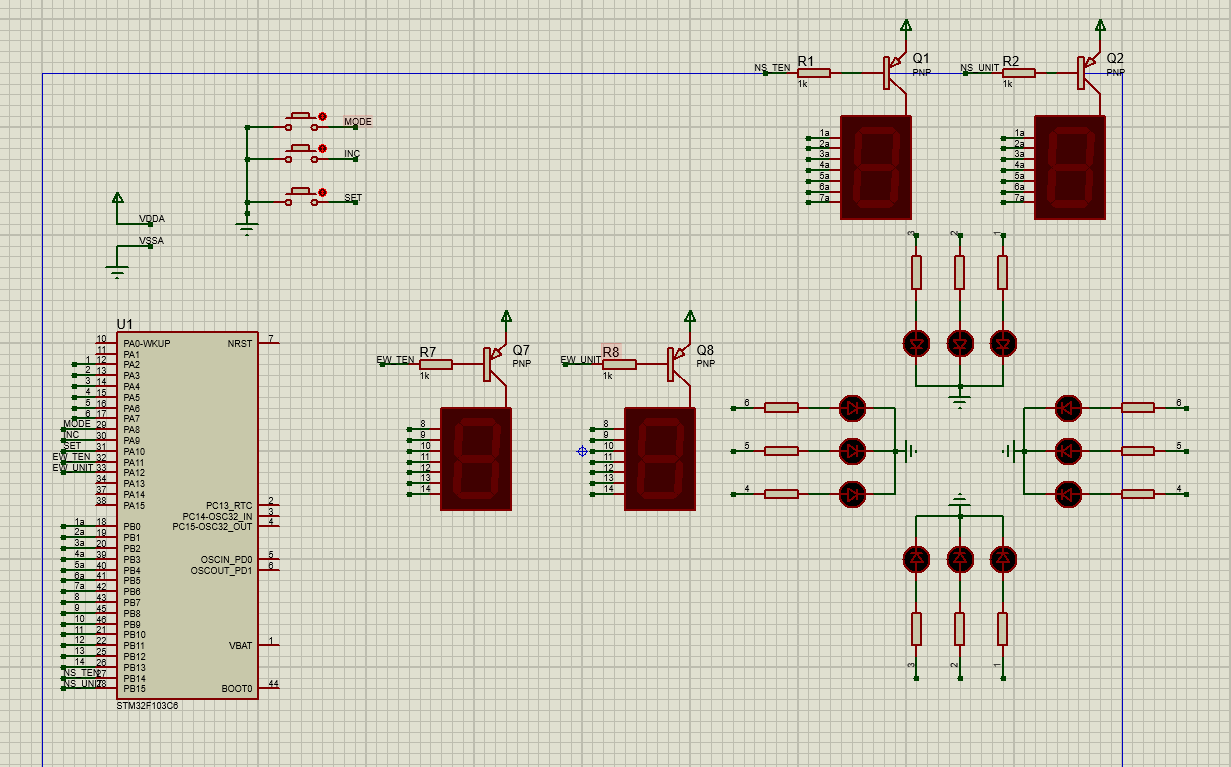
\includegraphics[width=\textwidth]{button.png}
\caption{Traffic-light schematic with MODE, INC, SET, and two display pairs.}
\label{fig:button}\end{figure}
\begin{table}[htbp]\centering
\caption{GPIO assignment used by the firmware and schematic}
\begin{tabular}{ll}\toprule
Function & GPIO assignment\\\midrule
NS red, amber, green & PA2, PA3, PA4\\
EW red, amber, green & PA5, PA6, PA7\\
MODE, INC, SET & PA8, PA9, PA10\\
NS segments a--g & PB0--PB6\\
EW segments a--g & PB7--PB13\\
NS tens, units enables & PB14, PB15\\
EW tens, units enables & PA11, PA12\\\bottomrule
\end{tabular}\end{table}

\topic{Shared commands and display buses}
Each road-pair color signal drives two LEDs in opposite approaches, accounting
for all twelve traffic LEDs. NS and EW have independent seven-wire segment
buses. Consequently, the scanner can enable the NS and EW tens simultaneously,
then enable both units simultaneously. The four displays require two scan slots,
not four. The transistor base resistors and traffic LED resistors shown in the
schematic belong to different circuit functions. The shared circuit is reused
for every later exercise, so additional schematic captures are unnecessary.

\topic{Electrical interpretation of an active-low button}

An open button must still produce a defined input level. With the internal
pull-up enabled, the released input is biased high. Pressing the switch connects
the pin to ground and the HAL read returns \code{GPIO_PIN_RESET}. Thus a
logical user action is obtained from a high-to-low electrical transition.
The pull-up establishes the idle voltage; software debouncing serves a different
purpose and does not replace that bias connection.

MODE, INC, and SET use separate pins, so the driver can sample all three in
one periodic loop without keyboard-matrix row selection. Their common ground
connection in Figure~\ref{fig:button} does not join the three signal nets.
Each input retains its own pull-up, sample history, and event counts.

\topic{Traffic and display current paths}

The traffic LEDs and display segments use opposite GPIO polarities.
For a traffic LED, a high command supplies its anode path through a series
resistor, while the cathode returns to ground. In each common-anode display,
the enabled PNP transistor supplies the common terminal and a low segment
output provides the return path. Pulling a PNP enable high removes that digit's
supply path. These connections explain why turning every traffic command low
switches the road LEDs off, whereas driving every segment high blanks a display.

The displayed pairs share segment signals only within their own road.
PB0--PB6 belong to NS and PB7--PB13 to EW. A segment update must use the
corresponding mask so it leaves the other road's data untouched. The two
remaining GPIOB pins select NS tens and units; PA11 and PA12 select EW tens
and units. PB3 and PB4 are used as segments, so their JTAG function must be
released while PA13 and PA14 can remain assigned to SWD.


\clearpage
\section{Exercise 3: STM32 project configuration}

\topic{Peripheral and module organization}
The MCU uses HSI at 8 MHz with no PLL and undivided AHB/APB clocks.
PA8--PA10 are input pins with \code{GPIO_PULLUP}; traffic, segment, and digit
enable signals are push-pull outputs. JTAG is disabled while SWD is retained,
freeing PB3 and PB4 for segment control. TIM2's global interrupt is enabled.
The runtime GPIO initialization, including user sections, defines the complete
pin allocation; generated configuration alone does not show every added pin.

The application is divided into \code{input_reading.c} for filtering/events,
\code{input_processing.c} for modes and phases, \code{output_display.c} for
GPIO/display conversion, and \code{timer.c} for periodic services.
Their matching headers expose public functions. \code{tim.c} initializes TIM2;
\code{stm32f1xx_it.c} routes SysTick and TIM2 interrupts to the application.
This division lets the FSM use button events and numerical display values
without repeating low-level GPIO operations.

\topic{CubeMX GPIO and pinout configuration}

Figure~\ref{fig:gpio} shows the configured pinout and input pull-ups. The three
button labels map directly to the event indices: index 0 is PA8/MODE, index 1
is PA9/INC, and index 2 is PA10/SET. Naming these pins makes the connection
between the circuit and the application's user interface easier to check.
The screenshot also shows the display enables at PA11--PA12 and PB14--PB15.

Initial traffic output levels are low. Segment outputs and PNP digit-enable
outputs start high so the displays remain blank while initialization is in
progress. Only after the output buffers and phase state have been established
does periodic scanning select a digit. Push-pull mode gives a defined driven
level for the output signals; input pull-up mode is used only for the buttons.

\begin{figure}[htbp]
\centering
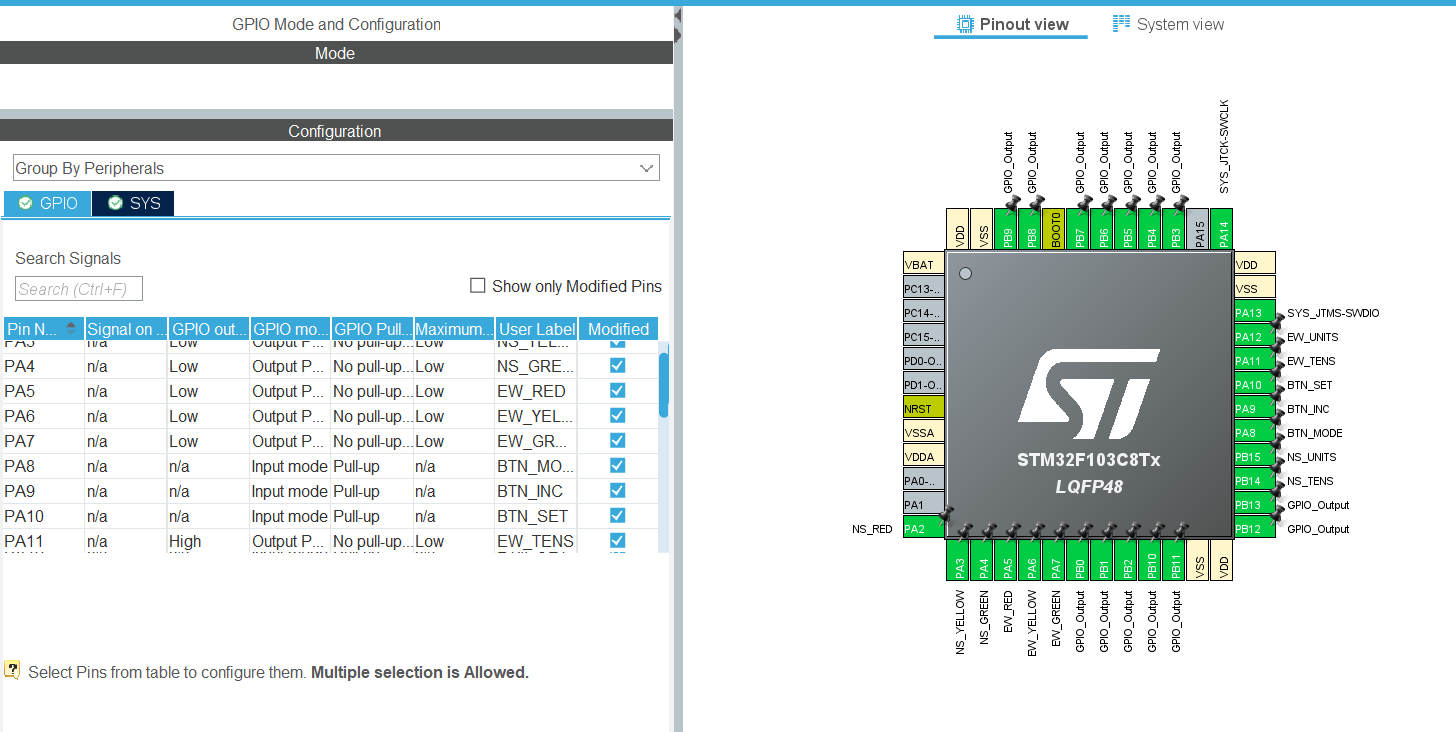
\includegraphics[width=\textwidth]{cubemx_gpio.png}
\caption{STM32CubeMX GPIO settings: active-low inputs with pull-ups and the project pinout.}
\label{fig:gpio}
\end{figure}

\topic{Ten-millisecond TIM2 calculation}
TIM2 receives 8 MHz. The prescaler 799 produces a 10-kHz counter clock.
With auto-reload 99, the counter takes 100 counts per interrupt:
\[
T_{\mathrm{TIM2}}=\frac{(799+1)(99+1)}{8\,000\,000}
=0.01\ \mathrm{s}=10\ \mathrm{ms}.
\]
The interrupt updates an elapsed-time value in milliseconds. SysTick remains
a separate 1-ms source for button sampling, display refresh, and setting-mode
blink scheduling. This project therefore uses two timing sources deliberately.

\begin{figure}[htbp]
\centering
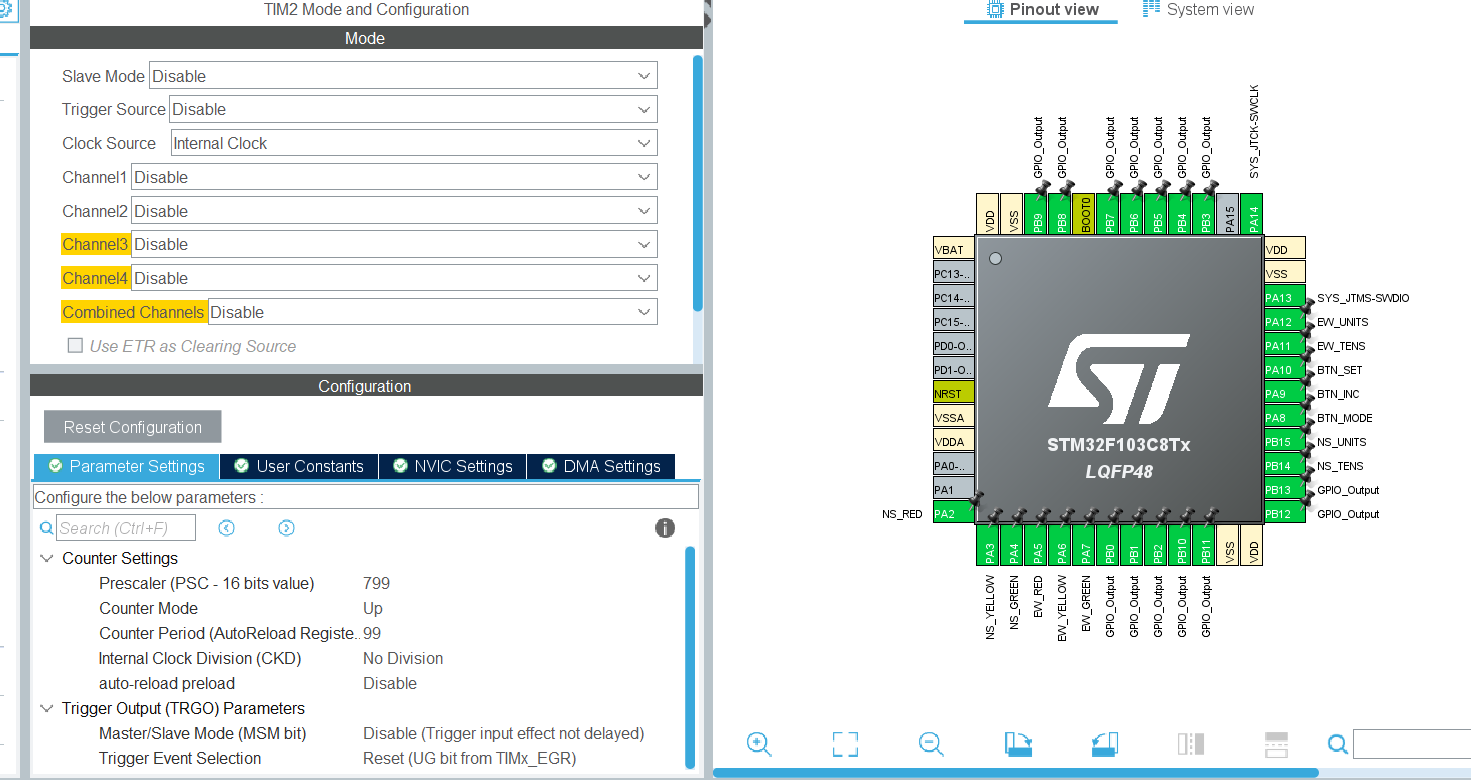
\includegraphics[width=\textwidth]{cubemx_tim2.png}
\caption{TIM2 internal-clock configuration: prescaler 799 and auto-reload 99.}
\label{fig:tim2}
\end{figure}
\topic{Interrupt enable and HAL event path}

The parameter values establish an update period but do not by themselves
guarantee execution of the application callback. The TIM2 clock must be enabled,
the global interrupt must be enabled in NVIC, the handler must call
\code{HAL_TIM_IRQHandler(&htim2)}, and the timer must be started with
\code{HAL_TIM_Base_Start_IT(&htim2)}. These stages connect the hardware
overflow event to \code{HAL_TIM_PeriodElapsedCallback()}.

Figure~\ref{fig:nvic} enables TIM2 with preemption priority 2. SysTick has
priority 15, so TIM2 has the higher urgency under this priority grouping.
The priority controls interrupt arbitration; it does not divide the timer clock
or change the requested 10-ms period. The callback checks the timer instance
before updating the TIM2-derived timestamp.

\begin{figure}[htbp]
\centering
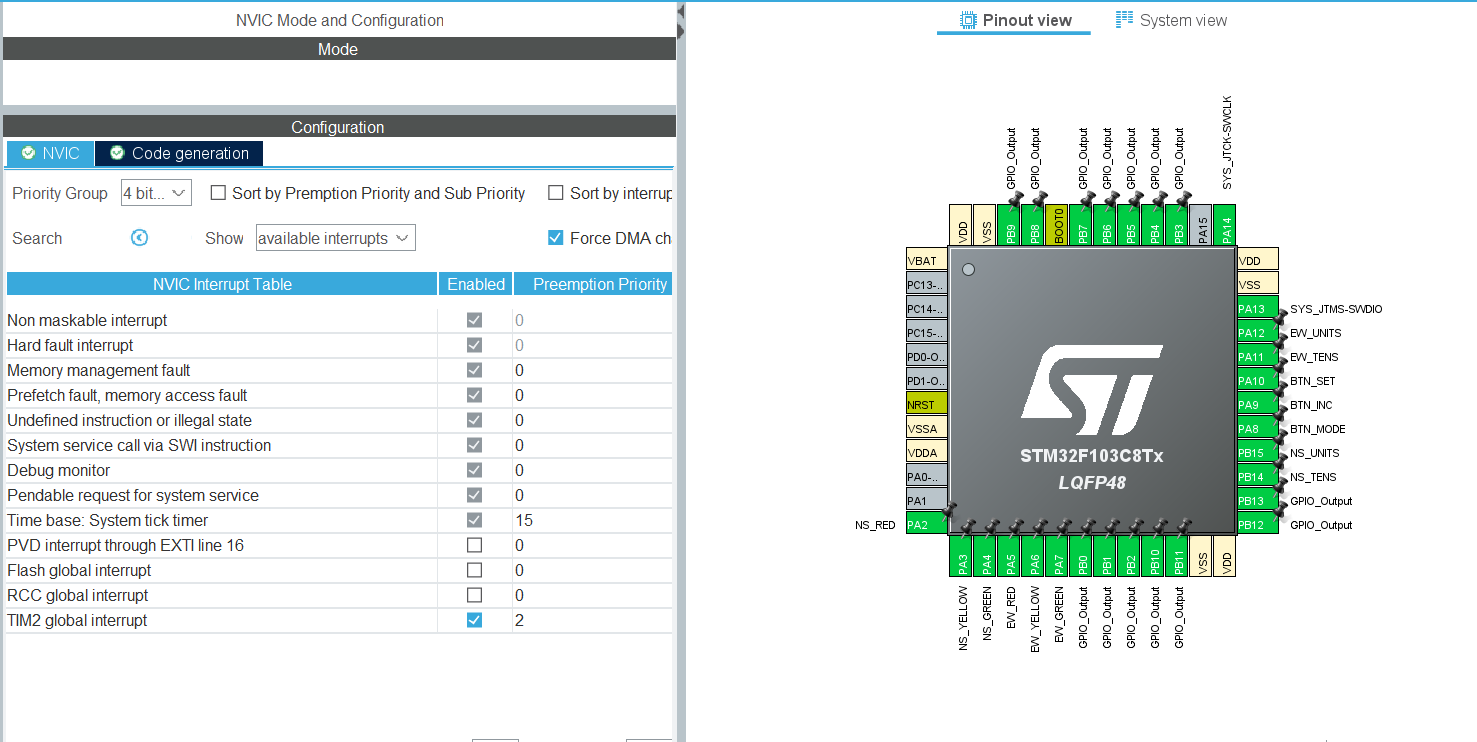
\includegraphics[width=\textwidth]{cubemx_nvic.png}
\caption{NVIC configuration: TIM2 interrupt enabled at priority 2 and SysTick at priority 15.}
\label{fig:nvic}
\end{figure}

\par\noindent\begin{minipage}{\linewidth}
\begin{lstlisting}[caption={Essential input pin configuration}]
GPIO_InitStruct.Pin = GPIO_PIN_8 | GPIO_PIN_9 | GPIO_PIN_10;
GPIO_InitStruct.Mode = GPIO_MODE_INPUT;
GPIO_InitStruct.Pull = GPIO_PULLUP;
HAL_GPIO_Init(GPIOA, &GPIO_InitStruct);
\end{lstlisting}
\end{minipage}\par

\topic{Clock-source verification and runtime initialization}

The firmware selects HSI directly, disables the PLL, and uses divide-by-one
prescalers for AHB and APB1. With APB1 undivided, the TIM2 clock equals the
8-MHz peripheral clock. A different clock-tree configuration would require
recalculating the timer parameters rather than copying the same numerical
values blindly\cite{rm0008}.

The CubeMX screenshot documents the initial 10-ms configuration. The project
also calls \code{timer_start()} after \code{MX_TIM2_Init()}. That function
reinitializes the timer using the application period macro. At the default
setting, its prescaler and auto-reload equal the screenshot values. When the
macro is changed for Exercise 4, the runtime initialization determines the
effective period. This distinction connects the configuration images to the
actual code path that starts the timer.


\clearpage
\section{Exercise 4: Changing the timer period}

\topic{Time units instead of fixed interrupt counts}
A task interval should be expressed in milliseconds rather than in a fixed
number of TIM2 invocations. \code{TIMER_CYCLE_MS} is the single period setting
used both to compute TIM2's auto-reload value and to advance application time.
With a 10-kHz timer clock, one millisecond contains ten counter increments:
\[
ARR=10T_{\mathrm{ms}}-1.
\]
For settings 1, 10, and 100 ms, ARR becomes 9, 99, and 999 respectively.
The callback adds 1, 10, or 100 ms to the timestamp rather than always adding
one. Normal countdown updates still compare elapsed time with 1000 ms.

\par\noindent\begin{minipage}{\linewidth}
\begin{lstlisting}[caption={Configurable TIM2 start sequence}]
void timer_start(void)
{
    ready = 0;
    time_ms = 0;
    button_counter = 0;
    scan_counter = 0;

    HAL_TIM_Base_Stop_IT(&htim2);
    htim2.Init.Prescaler = 799;
    htim2.Init.Period = TIMER_CYCLE_MS * 10 - 1;
    if (HAL_TIM_Base_Init(&htim2) != HAL_OK)
    {
        Error_Handler();
    }
    __HAL_TIM_SET_COUNTER(&htim2, 0);
    __HAL_TIM_CLEAR_FLAG(&htim2, TIM_FLAG_UPDATE);
    if (HAL_TIM_Base_Start_IT(&htim2) != HAL_OK)
    {
        Error_Handler();
    }

    ready = 1;
}
\end{lstlisting}
\end{minipage}\par

\par\noindent\begin{minipage}{\linewidth}
\begin{lstlisting}[caption={TIM2 elapsed-time service}]
void HAL_TIM_PeriodElapsedCallback(TIM_HandleTypeDef *htim)
{
    if (htim->Instance == TIM2)
    time_ms = time_ms + TIMER_CYCLE_MS;
}

uint32_t timer_get_time(void)
{
    return time_ms;
}
\end{lstlisting}
\end{minipage}\par

\topic{Parameter conversion and representative values}

The prescaled counter frequency remains
\(8\,000\,000/(799+1)=10\,000\) Hz, or one count every 0.1 ms.
A requested period of \(T\) milliseconds contains \(10T\) counts. Because
the counter includes zero, its last count is \(10T-1\), explaining the
minus one in the auto-reload calculation.
\begin{table}[htbp]\centering
\caption{TIM2 parameters for the three period choices}
\begin{tabular}{ccccc}\toprule
Period (ms) & PSC & ARR & Interrupt rate & Timestamp increment\\\midrule
1 & 799 & 9 & 1000 Hz & 1 ms\\
10 & 799 & 99 & 100 Hz & 10 ms\\
100 & 799 & 999 & 10 Hz & 100 ms\\\bottomrule
\end{tabular}\end{table}
For example, a 100-ms period needs ten TIM2 updates to account for one second,
whereas a 1-ms period needs one thousand. Both yield an elapsed timestamp
difference of 1000 ms. The application compares this difference with 1000,
so no traffic-phase threshold needs to be rewritten for those choices.

Stopping the timer before reinitialization avoids changing the active period
halfway through a running interval. The counter is reset and any pending update
flag is cleared before restarting. The time, scan, and input counters are also
initialized before the ready flag enables the SysTick-driven services.

\par\noindent\begin{minipage}{\linewidth}
\begin{lstlisting}[caption={Single application period selection in the timer header}]
#ifndef TIMER_CYCLE_MS
#define TIMER_CYCLE_MS 10
#endif
\end{lstlisting}
\end{minipage}\par

\topic{Keeping display and button intervals independent}
SysTick calls \code{HAL_IncTick()} and then \code{timer_tick_1ms()}.
Its scan counter triggers after five ticks; its button counter triggers after
ten ticks. Changing TIM2 to 100 ms therefore does not slow the display scanner
or the input filter. The ready flag prevents these services from executing
before initialization completes.

\par\noindent\begin{minipage}{\linewidth}
\begin{lstlisting}[caption={One-millisecond service scheduling}]
void timer_tick_1ms(void)
{
    if (ready == 0)
    {
        return;
    }

    scan_counter++;
    if (scan_counter >= 5)
    {
        scan_counter = 0;
        scan7SEG();
    }

    button_counter++;
    if (button_counter >= 10)
    {
        button_counter = 0;
        button_reading();
    }
}
\end{lstlisting}
\end{minipage}\par

\topic{Two-hertz blink calculation and timing resolution}
A 2-Hz blink means two complete ON--OFF cycles per second:
\[
T_{\mathrm{blink}}=500\ \mathrm{ms},\qquad
T_{\mathrm{toggle}}=250\ \mathrm{ms}.
\]
The implementation compares \code{HAL_GetTick()} with the previous blink
timestamp, so its 250-ms threshold is unaffected by the TIM2 period.
A design using only 100-ms ticks could not represent every 250-ms edge
exactly; the separate 1-ms SysTick avoids that limitation here.
TIM2 still determines the resolution of normal-road elapsed time. A changed
period preserves the 1000-ms nominal interval for the three specified settings,
but does not imply identical precision for every arbitrary duration.

\topic{Two time bases and foreground scheduling}

The HAL tick and the TIM2-derived time have the same unit, milliseconds, but
are not interchangeable variables. \code{HAL_GetTick()} is advanced by SysTick
every millisecond and is used for editing-mode blinking. \code{timer_get_time()}
returns application time accumulated by TIM2 and is used by the normal traffic
countdown. The button and scan counters are also maintained from SysTick.
This allocation preserves short user-interface intervals even when TIM2 is
configured for a coarse 100-ms period.

A blink comparison checks whether the elapsed HAL tick difference is at least
250 ms. The application then advances \code{last_blink} by 250 rather than
replacing it with the current time. This preserves the intended sequence of
nominal blink boundaries. Likewise, the normal second reference advances by
1000. Foreground execution still has to service these conditions promptly;
the calculations specify nominal schedule intervals, not independently
measured edge times.

For the default setting, a thousand SysTick ticks, one hundred TIM2 ticks,
two hundred display slots, and one hundred button-sampling calls all correspond
to one nominal second. Their counts differ because they serve different jobs,
not because the system maintains conflicting definitions of a second.


\clearpage
\section{Exercise 5: Button debouncing and mode events}

\topic{Three consecutive samples}
A mechanical press can produce alternating electrical levels before settling.
The driver stores three samples per button and accepts a new stable state only
when all three agree. Sampling every 10 ms places the first and third samples
20 ms apart. A sustained transition is normally accepted approximately
20--30 ms after its physical occurrence, depending on sample phase.
Short disturbances that do not create three matching samples are rejected.
Both press and release are filtered; a new press is recorded only when the
accepted state changes from high to low.

\begin{lstlisting}[caption={Button sampling, edge detection, and hold counting}]
void button_reading(void)
{
    int i;
    for (i = 0; i < 3; i++)
    {
        sample2[i] = sample1[i];
        sample1[i] = sample0[i];

        if (HAL_GPIO_ReadPin(GPIOA, button_pin[i]) == GPIO_PIN_RESET)
        sample0[i] = GPIO_PIN_RESET;
        else
        sample0[i] = GPIO_PIN_SET;

        if (sample0[i] == sample1[i] && sample1[i] == sample2[i])
        {

            if (stable[i] == GPIO_PIN_SET && sample0[i] == GPIO_PIN_RESET)
            press_count[i]++;

            stable[i] = sample0[i];
        }

        if (stable[i] == GPIO_PIN_RESET)
        {
            hold_counter[i]++;
            if (hold_counter[i] >= 150)
            {
                hold_counter[i] = 100;
                repeat_count[i]++;
            }
        }
        else
        {
            hold_counter[i] = 0;
        }
    }
}
\end{lstlisting}

\topic{Sample-by-sample debounce example}

Before a press, all three histories and the accepted state are high. On each
sample, the oldest history is discarded, the other two samples move back one
position, and a new GPIO reading enters \code{sample0}. A transition is
accepted only when \code{sample0}, \code{sample1}, and \code{sample2} agree.
\begin{table}[htbp]\centering
\caption{Example of rejecting a brief low pulse and accepting a sustained press}
\begin{tabular}{cccccc}\toprule
Sample & Raw & Newest & Previous & Oldest & Accepted state\\\midrule
Initial & 1 & 1 & 1 & 1 & Released\\
1 & 0 & 0 & 1 & 1 & Released\\
2 & 1 & 1 & 0 & 1 & Released\\
3 & 0 & 0 & 1 & 0 & Released\\
4 & 0 & 0 & 0 & 1 & Released\\
5 & 0 & 0 & 0 & 0 & Pressed; one event\\
6 & 0 & 0 & 0 & 0 & Pressed; no new event\\\bottomrule
\end{tabular}\end{table}
The low reading at sample 1 does not count as a press. Only the final three
consecutive lows at samples 3--5 establish the pressed state. Subsequent low
samples leave it pressed but do not create new press events, because edge
detection also requires the previous stable state to have been released.

The three matching observations span 20 ms, but their acceptance can occur
up to nearly one extra sampling period after a physical transition, giving
approximately 20--30 ms response for a clean sustained change. This is a
sampled filtering rule; it does not prove that no contact motion occurred
between observations. A release is accepted by the same three-high rule,
allowing a later press to generate a new high-to-low event.


\topic{Remembering and consuming events}
The three pin entries are PA8, PA9, and PA10. Sample and stable states are
initialized high, and event/hold counts begin at zero.
\code{press_count} records accepted presses; \code{handled_count} records
how many main has consumed. The consumer returns one event at a time while
the two counts differ. A press is consequently retained after the switch
has been released; it is not represented merely by the instantaneous level.
The listings retain this counting design without reproducing shared-state
declarations. The driver and FSM are separate modules.

\par\noindent\begin{minipage}{\linewidth}
\begin{lstlisting}[caption={Consuming a debounced press event}]
int button_pressed_event(int index)
{
    if (index < 0 || index > 2)
    {
        return 0;
    }

    if (handled_count[index] != press_count[index])
    {
        handled_count[index]++;
        return 1;
    }

    return 0;
}
\end{lstlisting}
\end{minipage}\par

\begin{lstlisting}[caption={Mode change and entry actions}]
static void change_mode(void)
{
    mode++;
    if (mode > 4)
    {
        mode = 1;
    }

    if (mode == 1)
    {
        start_normal();
    }
    else
    {
        if (mode == 2)
        {
            edit_value = red_time;
        }
        else if (mode == 3)
        {
            edit_value = yellow_time;
        }
        else
        {
            edit_value = green_time;
        }

        blink_on = 1;
        last_blink = HAL_GetTick();
        show_setting_lights();
        set_display(edit_value, mode);
    }
}
\end{lstlisting}

\topic{Event counts versus a pressed level}

A pressed level describes the present accepted switch state. A press event
describes a past transition that main has not yet consumed. Keeping counts
for the produced and handled events separates these meanings. If two distinct
accepted presses occur before main consumes them, the produced count advances
twice and the consumer can return two events over later foreground iterations.
Reading a button level directly would lose a completed short press if main
looked only after release.

For example, if \code{press_count[0]} is 4 and
\code{handled_count[0]} is 3, the next consumer call increments the handled
count to 4 and returns one. Another call then returns zero until a new event
is produced. The index check rejects negative indices and indices above two.
The repeat consumer uses the same pattern with separate counts. The sampling
driver therefore records input activity, while the foreground decides which
activity has meaning in the current mode.


\topic{Held INC behavior}
While the accepted button state is low, the hold counter increases once per
10-ms sample. The first repeat is generated at 150 samples, approximately
1.5 seconds after stable-press detection. The counter is then reset to 100;
another 50 samples produce the next repeat, giving 500-ms subsequent spacing.
The implemented threshold is 150 sampling calls, so the first repeat is
approximately 1.5 seconds rather than one second.
Only INC repeats are used by the FSM. MODE and SET repeats are consumed
without action, so holding MODE does not cycle through all modes.
Release resets the hold counter and a later press starts a new hold sequence.

\topic{Hold timing and why only INC repeats}

The first automatic increment is not the initial press event. A short INC
press already contributes one unit when its stable edge is accepted.
Continuing to hold the same press later generates repeat events. The hold
counter reaches its threshold on the 150th pressed-state sampling call, or
about 1.5 seconds on the 10-ms sampling scale. Resetting it to 100 instead
of zero makes the next threshold require only 50 further calls:
\[
T_{\mathrm{first\ repeat}}\approx150\times10=1500\ \mathrm{ms},
\qquad T_{\mathrm{repeat}}=(150-100)\times10=500\ \mathrm{ms}.
\]
The edge-acceptance sample also advances the hold counter, so these values
describe the nominal sampling count rather than an exact interval measured
from the physical contact closure. MODE and SET do not use automatic repeats:
holding MODE should not skip editing states, and holding SET should not keep
committing settings. Repeat events for those buttons are consumed without
changing the application state.

After an accepted release, the hold counter returns to zero. Filtering release
as well as press avoids restarting the held-button logic on a short unstable
sample. There is no foreground delay in the button interface, so the periodic
scanner and traffic FSM continue while the user presses or holds a switch.


\clearpage
\section{Exercise 6: Displaying modes and blinking the selected color}

\topic{Meaning of the two display pairs}
In normal mode, NS and EW show their respective remaining seconds.
In editing modes, NS shows \code{edit_value} and EW shows the two-digit
mode identifier: 02, 03, or 04. The setter updates numerical display buffers;
the scanner repeatedly converts tens with division by ten and units with
remainder by ten. This automatically displays leading zeros such as 05.
Negative display values select the middle segment to produce dashes.

\par\noindent\begin{minipage}{\linewidth}
\begin{lstlisting}[caption={Display-buffer update}]
void set_display(int ns, int ew)
{
    display_ns = ns;
    display_ew = ew;
}
\end{lstlisting}
\end{minipage}\par

\begin{lstlisting}[caption={Two-slot scanning of both road pairs}]
void scan7SEG(void)
{
    int ns = display_ns;
    int ew = display_ew;

    HAL_GPIO_WritePin(GPIOB, GPIO_PIN_14 | GPIO_PIN_15, GPIO_PIN_SET);
    HAL_GPIO_WritePin(GPIOA, GPIO_PIN_11 | GPIO_PIN_12, GPIO_PIN_SET);

    if (scan_index == 0)
    {
        if (ns < 0)
        {
            display7SEG(-1);
        }
        else
        {
            display7SEG(ns / 10);
        }

        if (ew < 0)
        {
            display7SEG_EW(-1);
        }
        else
        {
            display7SEG_EW(ew / 10);
        }

        HAL_GPIO_WritePin(GPIOB, GPIO_PIN_14, GPIO_PIN_RESET);
        HAL_GPIO_WritePin(GPIOA, GPIO_PIN_11, GPIO_PIN_RESET);
        scan_index = 1;
    }
    else
    {
        if (ns < 0)
        {
            display7SEG(-1);
        }
        else
        {
            display7SEG(ns % 10);
        }

        if (ew < 0)
        {
            display7SEG_EW(-1);
        }
        else
        {
            display7SEG_EW(ew % 10);
        }

        HAL_GPIO_WritePin(GPIOB, GPIO_PIN_15, GPIO_PIN_RESET);
        HAL_GPIO_WritePin(GPIOA, GPIO_PIN_12, GPIO_PIN_RESET);
        scan_index = 0;
    }
}
\end{lstlisting}

\topic{Decimal conversion and the two-slot sequence}

Each road value lies between 0 and 99 during normal display use. For a
nonnegative value \(v\), integer division gives the tens digit
\(\lfloor v/10\rfloor\) and remainder gives the units digit \(v\bmod10\).
Thus NS = 5 and EW = 2 become digits 0/5 and 0/2. If the editing mode is
red and its candidate is 12, the same scanner displays NS = 12 and EW = 02;
it does not need a separate mode-display driver.

In the tens slot, the NS bus is loaded with its tens pattern and the EW bus
with its own tens pattern. PB14 and PA11 are then pulled low together.
In the units slot, those enables are first switched off, the two unit patterns
are prepared, and PB15/PA12 are enabled. Only one digit per bus is active,
although two physical digits are active across the whole circuit. The two
buses are the reason four physical digits require only two time slots.

Before a pattern changes, all four digit enables are driven high. This
break-before-make order prevents the old digit from briefly showing the new
digit's pattern, commonly called ghosting. The brief blanking time is small
compared with the 5-ms slot. A negative display value follows a separate
branch that lights only the middle segment, allowing both pairs to show
dashes when normal timing is invalid.


\topic{Refresh frequency and output polarity}
One slot lasts 5 ms. Since the two independent buses allow both tens to be
selected together, the full frame has two slots:
\[
T_{\mathrm{frame}}=2\times5=10\ \mathrm{ms},\qquad
f_{\mathrm{frame}}=100\ \mathrm{Hz}.
\]
Each digit has approximately 50\% duty cycle, apart from switching overhead.
The scanner disables all PNP enables before changing segment data, reducing
unwanted patterns during transitions. Traffic outputs are handled separately:
all six commands are cleared before the selected active-high color mask is set.

\par\noindent\begin{minipage}{\linewidth}
\begin{lstlisting}[caption={Traffic outputs and setting-color selection}]
void TrafficLight_Init(uint16_t ns_led, uint16_t ew_led)
{
    HAL_GPIO_WritePin(GPIOA, ALL_TRAFFIC_LEDS, GPIO_PIN_RESET);
    if (ns_led != 0 || ew_led != 0)
    HAL_GPIO_WritePin(GPIOA, ns_led | ew_led, GPIO_PIN_SET);
}

static void show_setting_lights(void)
{
    if (blink_on == 0)
    TrafficLight_Init(0, 0);
    else if (mode == 2)
    TrafficLight_Init(NS_RED, EW_RED);
    else if (mode == 3)
    TrafficLight_Init(NS_YELLOW, EW_YELLOW);
    else if (mode == 4)
    TrafficLight_Init(NS_GREEN, EW_GREEN);
}
\end{lstlisting}
\end{minipage}\par

\topic{Blink state and expected sequence}
Entering an editing mode sets \code{blink_on} to one and records the current
HAL tick. After 250 ms it changes to zero, and after another 250 ms it changes
back to one. In mode 2 all four red LEDs blink; modes 3 and 4 similarly blink
all amber or green LEDs. Other colors are off. Mode and candidate displays
remain refreshed during both ON and OFF intervals. A new mode entry begins
with its selected color on rather than inheriting an arbitrary blink phase.

\par\noindent\begin{minipage}{\linewidth}
\begin{lstlisting}[caption={Setting-mode blink scheduling}]
if (HAL_GetTick() - last_blink >= 250)
{
    last_blink = last_blink + 250;
    if (blink_on == 1)
    {
        blink_on = 0;
    }
    else
    {
        blink_on = 1;
    }
    show_setting_lights();
}
set_display(edit_value, mode);
\end{lstlisting}
\end{minipage}\par

\topic{Frequency, duty cycle, and user-visible behavior}

At the 5-ms slot interval, the selection function is called 200 times per
second, but each physical digit is revisited 100 times per second. The complete
frame frequency is therefore 100 Hz, not 200 Hz. Tens and units each receive
approximately half of the available on-time. Changing the numerical candidate
updates a buffer immediately in main; the next scan slots display the new
tens and units without stopping the refresh service.

The editing-color blink has a much slower time scale. Starting ON at mode
entry, the selected LEDs are OFF at nominal 250 ms, ON at 500 ms, OFF at
750 ms, and ON again at 1000 ms. There are four state changes but only two
complete cycles in that second. The seven-segment display does not follow
\code{blink_on}; it stays refreshed while the traffic color is in either
its ON or OFF half-cycle. This gives visible mode feedback without hiding the
candidate value during the dark portion of a blink.


\clearpage
\section{Exercise 7: Adjusting the red duration}

\topic{Candidate adjustment and range}
MODE enters state 2 and copies the committed red duration into the candidate.
Each accepted INC event adds one; holding INC generates further increases
after the hold interval described in Exercise 5. Values cycle through 1--99.
The active duration is not overwritten by INC alone, so an unconfirmed value
can be inspected on NS while EW displays 02.

\par\noindent\begin{minipage}{\linewidth}
\begin{lstlisting}[caption={Shared candidate increment in modes 2--4}]
if (button2 == 1)
{
    edit_value++;
    if (edit_value > 99)
    {
        edit_value = 1;
    }
}
\end{lstlisting}
\end{minipage}\par

\topic{Commit rule and worked example}
The implemented policy retains amber and derives green from the new red:
\(G_{\mathrm{new}}=R_{\mathrm{new}}-Y\).
Therefore a red candidate is accepted only when it exceeds amber, ensuring
positive green time. If rejected, the displayed candidate returns to the
previous committed red value. SET commits within mode 2 and does not itself
return to normal operation.
The handout permits 1--99 as the editing range; the positivity and timing
relation further restrict the values that this implementation can commit.

\par\noindent\begin{minipage}{\linewidth}
\begin{lstlisting}[caption={SET action for mode 2}]
if (mode == 2)
{
    if (edit_value > yellow_time)
    {
        red_time = edit_value;
        green_time = red_time - yellow_time;
    }
    else
    {
        edit_value = red_time;
    }
}
\end{lstlisting}
\end{minipage}\par

\topic{Red-mode event trace and valid commit range}

The red candidate can be increased through the entire editing range 1--99,
but the commit condition imposes a stricter relation. With fixed amber Y,
the valid committed red values are
\[
Y+1\le R_{\mathrm{new}}\le99.
\]
The lower limit guarantees \(G_{\mathrm{new}}\ge1\). Because Y is positive,
the resulting green value is also below 99. The code therefore preserves
positive two-digit durations while maintaining the phase timing relation.

With the defaults, MODE enters red editing and displays 05/02. One INC
changes the candidate display to 06/02 while the committed configuration is
still (5,2,3). Pressing SET makes it (6,2,4), and the candidate remains 6.
If MODE is pressed before SET, no red update occurs. A candidate can also
wrap from 99 to 1; with amber 2, pressing SET on 1 fails validation and
restores candidate 5 if the committed red time is still the default.

Red is the user's selected duration, amber is preserved, and green is the
dependent duration. This commit policy maintains the two-road phase model.


\clearpage
\section{Exercise 8: Adjusting the amber duration}

\topic{Mode entry and shared editing algorithm}
The next MODE event enters mode 3, loads the current amber duration, and
displays the candidate on NS with 03 on EW. All four amber LEDs blink at 2 Hz.
The INC/wrap function is exactly the shared block in Exercise 7. Reusing it
ensures that all editing modes apply the same one-step and held-repeat behavior.

\topic{Commit rule and worked example}
Amber editing preserves red and derives green:
\(G_{\mathrm{new}}=R-Y_{\mathrm{new}}\).
The candidate must be less than red; equality would make green zero and a
larger value would make it negative. An invalid candidate is replaced by the
old amber value without changing the committed configuration.
For \((5,2,3)\), increasing amber to 3 and pressing SET gives \((5,3,2)\).
The complete cycle remains ten seconds, but each green interval is shorter
and each amber interval longer. This explains why committing one color may
change another duration in the current implementation.

\par\noindent\begin{minipage}{\linewidth}
\begin{lstlisting}[caption={SET action for mode 3}]
else if (mode == 3)
{
    if (edit_value < red_time)
    {
        yellow_time = edit_value;
        green_time = red_time - yellow_time;
    }
    else
    {
        edit_value = yellow_time;
    }
}
\end{lstlisting}
\end{minipage}\par

\topic{Amber-mode constraints and countdown consequences}

For a fixed committed red time R, acceptable amber candidates satisfy
\[
1\le Y_{\mathrm{new}}\le R-1,\qquad
G_{\mathrm{new}}=R-Y_{\mathrm{new}}.
\]
The strict inequality in the code ensures there is still at least one second
of green. Red is preserved by this editing policy, so the complete normal
cycle \(2R\) remains constant even though the green/amber division changes.

Starting from (5,2,3), mode 3 initially shows 02/03. One INC selects 03/03,
and SET commits (5,3,2). When normal operation is restarted, NS green lasts
2 s and NS amber lasts 3 s. EW stays red for the combined 5 s. At entry to
the amber phase, both countdowns are loaded with 3, because EW's red interval
has 3 s remaining. This example connects the configuration update directly
to the two countdown displays in the phase machine.

A candidate equal to 5 with red 5 is rejected, and its displayed value is
restored to the committed amber time. The red and green values are not partly
updated on that rejected branch. As in the other modes, a held INC can select
values faster, while SET remains a one-press confirmation and the amber
blink continues independently throughout the interaction.


\clearpage
\section{Exercise 9: Adjusting the green duration}

\topic{Mode entry and confirmation}
MODE next enters mode 4, which displays the green candidate and mode 04.
All four green LEDs blink. INC changes only the candidate using the same
1--99 wrap rule. SET preserves amber and computes the necessary red duration:
\(R_{\mathrm{new}}=G_{\mathrm{new}}+Y\).
The sum must not exceed 99 because each road has only two decimal positions.
For a fixed amber value Y, the largest acceptable green value is \(99-Y\).

\par\noindent\begin{minipage}{\linewidth}
\begin{lstlisting}[caption={SET action for mode 4}]
else if (mode == 4)
{
    if (edit_value + yellow_time <= 99)
    {
        green_time = edit_value;
        red_time = green_time + yellow_time;
    }
    else
    {
        edit_value = green_time;
    }
}
\end{lstlisting}
\end{minipage}\par

\topic{Worked example and return to normal}
Starting at \((5,2,3)\), two INC events select green 5. SET commits
\((7,2,5)\), so one complete normal cycle lasts fourteen seconds.
With amber 2, a green candidate 98 is rejected because red would need 100.
The previous green value is restored on the display.
After the next MODE press, state 4 wraps to state 1. Normal operation restarts
from NS green/EW red with the committed durations; it does not resume the
countdown at the point where editing was entered. Since there is no persistent
storage operation, a reset initializes the default 5/2/3 configuration again.

\topic{Green-mode range and complete-cycle calculation}

Green editing preserves amber rather than red. The upper bound follows from
the two-digit maximum of the derived red interval:
\[
1\le G_{\mathrm{new}}\le99-Y,\qquad
R_{\mathrm{new}}=G_{\mathrm{new}}+Y,\qquad
T_{\mathrm{cycle,new}}=2(G_{\mathrm{new}}+Y).
\]
For amber 2, the maximum acceptable green value is 97. Green 97 produces
red 99, so all display values remain within two digits. Green 98 would
require red 100 and is rejected; a candidate being within 1--99 alone does
not guarantee that its related red duration fits the display.

For the example (5,2,3), selecting green 5 gives red 7 after confirmation.
Normal phases then last 5, 2, 5, and 2 seconds. At phase-zero entry the
displays are 05/07. After five seconds phase 1 displays 02/02, and after
seven seconds phase 2 displays 07/05. This makes the new fourteen-second
cycle understandable from both the color outputs and their countdowns.


\clearpage
\section{Exercise 10: Integrated traffic-light application}

\topic{Initialization and foreground loop}
HAL and clock initialization precede GPIO and TIM2 configuration.
Input initialization establishes released samples and empty event counts.
Output initialization disables digit enables and commands both roads red.
FSM initialization loads the default durations and starts phase 0.
Finally, timer initialization enables periodic operation. The main loop
repeatedly processes button events and state actions without a blocking delay.

\par\noindent\begin{minipage}{\linewidth}
\begin{lstlisting}[caption={Essential application initialization and main loop}]
HAL_Init();
SystemClock_Config();
MX_GPIO_Init();
MX_TIM2_Init();
input_init();
output_init();
fsm_init();
timer_start();

while (1)
{
    fsm_run();
}
\end{lstlisting}
\end{minipage}\par

\topic{Event dispatch and priority}
Each iteration obtains one pending event from each button. INC repeat events
are merged into the increment request, while repeat events for the other
buttons are discarded. MODE is handled first. In normal mode, INC and SET
events are consumed without modifying durations. In an editing mode, the
shared INC block, mode-specific SET block, blink update, and display-buffer
update execute in that order.

\par\noindent\begin{minipage}{\linewidth}
\begin{lstlisting}[caption={Core event dispatch at the start of the FSM}]
int button1 = button_pressed_event(0);
int button2 = button_pressed_event(1);
int button3 = button_pressed_event(2);

if (button_repeat_event(1) == 1)
{
    button2 = 1;
}
button_repeat_event(0);
button_repeat_event(2);

if (button1 == 1)
{
    change_mode();
    return;
}

if (mode == 1)
{
    normal_run();
}
\end{lstlisting}
\end{minipage}\par

\topic{One-second countdown and phase transitions}
Normal operation compares the TIM2-derived timestamp with the previous
second boundary. Advancing the previous timestamp by 1000 instead of replacing
it with the current time preserves the intended sequence of second boundaries.
If foreground processing is temporarily late, successive loop iterations can
process outstanding seconds. Each second decrements both road countdowns.
Only the active green/amber road determines when the next phase begins.

\begin{lstlisting}[caption={Normal operation and countdown transitions}]
static void normal_run(void)
{
    if (red_time != green_time + yellow_time)
    {
        return;
    }

    if (timer_get_time() - last_second >= 1000)
    {
        last_second = last_second + 1000;
        ns_count--;
        ew_count--;

        if ((phase == 0 || phase == 1) && ns_count == 0)
        {
            phase++;
            show_phase();
        }
        else if ((phase == 2 || phase == 3) && ew_count == 0)
        {
            phase++;
            if (phase > 3)
            {
                phase = 0;
            }
            show_phase();
        }

        set_display(ns_count, ew_count);
    }
}
\end{lstlisting}

\topic{Expected normal sequence}
With the default settings, phase 0 begins at NS 03/EW 05. After one second,
the displays become 02/04; after two seconds, 01/03. At three seconds the
controller enters phase 1 and loads 02/02. At five seconds it enters phase 2,
loading 05/03. At eight seconds phase 3 loads 02/02. At ten seconds phase 0
begins again. Zero is used as a transition condition rather than held for an
extra one-second interval.

The start routine checks \(R=G+Y\) before enabling the sequence. If this
relationship is violated, both roads remain red and the displays show dashes.
The normal update routine also refuses to advance an inconsistent configuration.
The commit rules of Exercises 7--9 normally preserve the relationship.

\topic{Integrated default cycle, second by second}

The following values are expected immediately after foreground handling of
each nominal one-second boundary. The brief transient value zero is used to
detect a phase end and is replaced by the next phase's entry counts in the
same update operation.
\begin{table}[htbp]\centering
\caption{Expected default normal-mode sequence over ten seconds}
\begin{tabular}{cccll}\toprule
Time (s) & Phase & NS / EW displays & NS color & EW color\\\midrule
0 & 0 & 03 / 05 & Green & Red\\
1 & 0 & 02 / 04 & Green & Red\\
2 & 0 & 01 / 03 & Green & Red\\
3 & 1 & 02 / 02 & Amber & Red\\
4 & 1 & 01 / 01 & Amber & Red\\
5 & 2 & 05 / 03 & Red & Green\\
6 & 2 & 04 / 02 & Red & Green\\
7 & 2 & 03 / 01 & Red & Green\\
8 & 3 & 02 / 02 & Red & Amber\\
9 & 3 & 01 / 01 & Red & Amber\\
10 & 0 & 03 / 05 & Green & Red\\\bottomrule
\end{tabular}\end{table}
The two road displays are not independent timers that change traffic colors
on their own. Both are updated by a single phase transition. This is why the
opposing countdown is reloaded consistently when one road changes from green
to amber. One shared phase variable determines the compatible pair of outputs.

\topic{Startup, foreground latency, and re-entry behavior}

During startup, the input histories are initialized before sampling is enabled.
Output initialization blanks the PNP enables and prepares numerical buffers.
FSM initialization selects mode 1, sets durations to 5/2/3, and enters phase 0.
Starting the timers last ensures the periodic services do not read application
state before these initial values have been established.

The normal elapsed-time test uses a millisecond difference and advances the
stored reference by 1000 for each processed second. If a short foreground
delay leaves the timestamp more than one second ahead, repeated main-loop
iterations can process the overdue second boundaries. Each call processes
at most one second because the implementation uses an \code{if} rather
than an inner catch-up loop. This scheduling property does not make delayed
physical color transitions retroactive; the intended operation relies on a
foreground loop that remains responsive.

Editing does not decrement the suspended normal countdowns. Re-entering mode 1
records the current application time as the new reference and starts phase 0.
Consequently, time spent adjusting a candidate does not appear as a burst of
old traffic-phase updates on return. Accepted settings are stored in RAM only;
the initialization function restores defaults at reset. No flash-save feature
is implied by the SET action.


\topic{Demonstration sequence}
A demonstration of the integrated application should show a complete normal
cycle and the two simultaneous road countdowns, then use MODE to visit 02,
03, and 04. In each editing mode, the selected color should complete two
ON--OFF cycles per second while the candidate and mode remain visible.
Show a short INC press, a held INC operation, the 99-to-1 wrap, and a SET
confirmation. Return to mode 1 to show the revised timing in operation.
An invalid red/amber relationship and a green value whose sum exceeds 99
can demonstrate the rejection rules. Reset demonstrates restoration of defaults.
These observations describe the expected application behavior. The video
demonstration should present them together with the displayed mode and values.

\section*{Conclusion}
\addcontentsline{toc}{section}{Conclusion}
The controller combines debounced input events, a mode FSM, a traffic-phase
FSM, and multiplexed numerical output. Three matching input samples distinguish
a stable action from short contact changes, while event counts separate input
detection from foreground consumption. Candidate values and SET confirmation
provide controlled editing of the traffic durations.

Millisecond-based scheduling separates user-visible intervals from the TIM2
interrupt count. SysTick maintains fast button and display services while TIM2
provides normal-operation elapsed time. Two simultaneous display buses allow a
100-Hz complete two-slot refresh, and 250-ms color transitions implement 2-Hz
editing-mode blinking. The relation R = G + Y coordinates opposing roads,
and explicit phase transitions prevent conflicting green commands in normal
operation. These mechanisms form a complete non-blocking user interface for
configurable traffic-light timing.
\clearpage
\phantomsection
\addcontentsline{toc}{section}{References}
\begin{thebibliography}{5}
\bibitem{stm32}
STMicroelectronics, ``STM32F103 product family,'' product documentation.
Available from the
\href{https://www.st.com/en/microcontrollers-microprocessors/stm32f103.html}
{STMicroelectronics STM32F103 product page}.
Accessed: November 4, 2026.

\bibitem{hal}
STMicroelectronics, \emph{Description of STM32F1 HAL and Low-Layer Drivers},
User Manual UM1850. Available from the
\href{https://www.st.com/resource/en/user_manual/um1850-description-of-stm32f1-hal-and-lowlayer-drivers-stmicroelectronics.pdf}
{STMicroelectronics document archive}.
Accessed: November 4, 2026.

\bibitem{keil}
Arm Keil, ``\mbox{$\mu$Vision} User's Guide.'' Available from the
\href{https://www.keil.com/support/man/docs/uv4/default.htm}
{Keil documentation website}.
Accessed: November 4, 2026.

\bibitem{proteus}
Labcenter Electronics, ``Proteus Design Suite: PCB design and circuit simulation
software.'' Available from the
\href{https://www.labcenter.com/}{Labcenter Electronics website}.
Accessed: November 4, 2026.
\bibitem{rm0008}
STMicroelectronics, \emph{STM32F101xx, STM32F102xx, STM32F103xx,
STM32F105xx and STM32F107xx advanced Arm-based 32-bit MCUs},
Reference Manual RM0008. Available from the
\href{https://www.st.com/resource/en/reference_manual/cd00171190-stm32f101-103-105-107-stm32f100-series-armbased-32bit-mcus-stmicroelectronics.pdf}
{STMicroelectronics reference-manual archive}.
Accessed: November 4, 2026.
\end{thebibliography}
\end{document}
